% brainstorm:

% * revisão das teorias de contornos
% * parte da análise que fiz do opus 5 mov 3 de Webern
% * exemplos de usos de operações na peça do mestrado e experimentos
% * desenvolvimento do goiaba (para que serve e um exemplo da saída)

\section{Introduction}
\label{sec:introduction}

Contour can be defined as a object profile or shape. It can be
bidimensional and associate a dimension like height to another like
time. It can be also multidimensional, and associate three or more
dimensions, like height and length to time. In this paper we use only
bidimensional contours. In music, contours can be associated to pitch,
density, rhythm, rhythmic complexity, orchestral homogeneity,
intensity, etc. Melodic contours are related to pitch movement as
function of time. For instance, Beethoven's Fifth Symphony main motive
and its contour are represented respectively in figures
\ref{fig:5a-sinfonia-motivo} and \ref{fig:c-3120}.

\begin{figure}[!p]
  \centering
  \subfloat[Main motive]{
    \includegraphics{5a-sinfonia}
    \label{fig:5a-sinfonia-motivo}
  }
  \subfloat[Contour (3 1 2 0)]{
    \includegraphics{c-3120}
    \label{fig:c-3120}
  }
  \caption{Fifth Symphony main motive contour}
  \label{fig:5a-sinfonia}
\end{figure}

Contour study is important because, like motives and pitch sets,
contours can help to give coherence to a musical piece. They represent
handling musical structures through operations like inversion and
retrogradation, and can be aproached by analytical or compositional
points of view.

Despite the possible coherence given by contours and the operations
provided by contour theories, systematic studies of contour operations
and combinations usage in musical composition are scarce. It's
necessary experimentation and studies about this operations usage in
composition area.

In this paper we present a brief review of contour literature, a
contour analytic usage example, and contour applications in
composition. This paper represents a short summary of the
compositional contour applications research now in progress and
described in Sampaio master's thesis \cite{sampaio08:em}.

\section{Contour theories}
\label{sec:contour-theories}

Many authors
\cite{friedmann85:methodology,friedmann87:response,morris87:composition,morris93:directions,marvin.ea87:relating,marvin88:generalized,marvin.ea95:generalization,polansky.ea92:possible,quinn97:fuzzy,clifford95:contour,beard03:contour}
have developed theories to system the contour study. These theories
were developed primarily as analytic techniques for non-tonal
compositions without typical musical features used to demonstrate
coherence in tonal compositions, like phrase, periods, themes and
functional analysis \cite{beard03:contour}.

These theories provides arrays, matrixes and many operations to help
in comparing contours, like inversion, translation, contour elements
comparison, and contour similarity comparisons, comparison matrix and
contour interval array.

Music analysis under contour point of view have been effective in
tonal and non-tonal music. There are successful analysis of A.
Schoenberg \cite{friedmann85:methodology}, A. Webern
\cite{clifford95:contour}, L. Dallapicolla
\cite{marvin88:generalized}, and W. A. Mozart \cite{beard03:contour}
pieces. Clifford \cite{clifford95:contour}, for example, says contour
has a significant role in Webern pre-serial music structure.

The compositional contour applications research said is based in these
theories. Two short pieces and an eleven minutes woodwind quintet were
composed based on combinated contour operations to experiment contour
possibilities in composition. A contour processor software is been
developed as main object of Sampaio doctor's. This software, called
\goiaba{}\footnote{\url{http://genos.mus.br/goiaba/}}, receives
symbollic contours as input and outputs symbollic and graphical
representations of contours and operations. In future \goiaba{} will
receive Lilypond\footnote{\url{http://lilypond.org/}} format scores
input and will have a graphical interface.

\section{Music Analysis}
\label{sec:music-analysis}

\begin{figure}[!p]
  \centering
  \subfloat[Theme contours]{
    \includegraphics{webern-tema-analisado}
    \label{fig:webern-tema-analisado}
  }

  \subfloat[Contour concatenation]{
    \includegraphics{webern-concatenacao-1}
    \label{fig:webern-concatenacao-1}
  }
  \quad
  \subfloat[Contour concatenation]{
    \includegraphics{webern-concatenacao-2}
    \label{fig:webern-concatenacao-2}
  }
  \caption{Contours in Webern Op.5, mov.3}
  \label{fig:exemplos-webern}
\end{figure}


\section{Contour in Composition}
\label{sec:contour-composition}

Sampaio master's thesis main result \cite{sampaio08:em} was a
composition based on contours operations combinations.

This piece is based on a six notes motive called $\alpha$
(fig. \ref{fig:motivo-alfa}) and its derived contour P(5 3 4 1 2
0). This motive is based on octatonic scale.

\begin{figure}[!p]
  \centering
  \subfloat[$\alpha$ motive]{
    \includegraphics{motivo-alfa}
    \label{fig:motivo-alfa}
  }
  \subfloat[P(5 3 4 1 2 0) contour]{
    \includegraphics{c-534120}
    \label{fig:c-534120}
  }
  \caption{Materials}
  \label{fig:materials}
\end{figure}

In the piece there is a \eng{fugato}. The subject and countersubject
are based on rotation and retrogradation operations. The subject has
original contour P(5 3 4 1 2 0) and factor 3 rotation
(fig. \ref{fig:sujeito-fugato}). The contoursubject has original
contour retrogradation repeated three times with different rotation
factors---5, 4 and 3 (fig. \ref{fig:contra-sujeito-fugato}).

\begin{figure}
  \centering
  \subfloat[Subject]{
    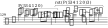
\includegraphics[scale=3.2]{sujeito-fugato}
    \label{fig:sujeito-fugato}
  }

  \subfloat[Countersubject]{
    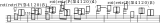
\includegraphics[scale=3.2]{contra-sujeito-fugato}
    \label{fig:contra-sujeito-fugato}
  }
  \caption{Structural elements of \eng{fugato}}
  \label{fig:elementos-fugato}
\end{figure}

Contours were divided in smaller pieces by interval expanded
interpolated contours. In figure \ref{fig:interpolacao-expansao},
contour Q(0 2 1 4 3 5) has G, B$\flat$ A, C$\sharp$, B$\sharp$ and
D$\sharp$ long notes and is divided in two pieces by the interval
expanded interpolated contour with C$\sharp$, G, E, B$\flat$, G and
C$\sharp$ short notes.

\begin{figure}[!p]
  \centering
  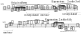
\includegraphics[scale=4.8]{oboe-solo-secao-5}
  \caption{Interpolation and expansion}
  \label{fig:interpolacao-expansao}
\end{figure}

Rotation and interval expansion occur like in figure
\ref{fig:notas-curtas-madeiras}. In flute the contour has original
form, and in clarinet there is a factor 2 rotation and an
expansion. In oboe there is a factor 3 rotation and contour deviation
justified by the gesture. In bassoon there is a factor 3 contour
rotation and retrogradation, and intervallic expansion.

\begin{figure}[!p]
  \centering
  \subfloat[4 fragments composed by rotation and expansion]{
    \includegraphics[scale=1]{notas-curtas-madeiras}
    \label{fig:notas-curtas-madeiras}
  }

  \subfloat[original]{
    \includegraphics[scale=.75]{c-534120}
    \label{fig:rot-0}
  }
  \subfloat[rot 2]{
    \includegraphics[scale=.75]{c-412053}
    \label{fig:rot-2}
  }
  \subfloat[rot 3]{
    \includegraphics[scale=.75]{c-120534}
    \label{fig:rot-3}
  }
  \subfloat[retr(rot 3)]{
    \includegraphics[scale=.75]{c-435021}
    \label{fig:rot-3-retr}
  }
  \caption{Rotation and expansion}
  \label{fig:rotacao-expansao}
\end{figure}

The second section of the piece has pitch amplitude grown and raised
by P(5 3 4 1 2 0) contour expansion. Notes are choosen in octatonic
scale omitting one note in each three. Figure ilustrates this
process. In G F$\sharp$ E D$\sharp$ C$\sharp$ C$\natural$ B$\flat$ A G
F$\sharp$ E scale the notes F$\sharp$, D$\sharp$, C$\natural$, A, and
F$\sharp$ are ommitted, the remain notes G, E, C$\sharp$, B$\flat$, G,
E, and are kept and ordered in contour resulting G C$\sharp$ E G
B$\flat$ E. This procedure is repeated omitting two adjacent notes in
each four, omitting three adjacent notes in each five and so on.

\begin{figure}[!p]
  \centering
  \subfloat[Process to choose notes: omitting one note]{
    \includegraphics[scale=.8]{escala-secao-2-one}
    \label{fig:escala-expansao-omissao}
  }

  \subfloat[Analytic reduction of expansion usage]{
    \includegraphics[scale=.8]{secao-2}
    \label{fig:secao-2-reduction}
  }
  \caption{Expansion process}
\end{figure}

\section{Conclusions}
\label{sec:conclusions}

%%% Local Variables: 
%%% mode: latex
%%% TeX-master: "contour-composition"
%%% End: 